\documentclass[10pt]{dokument-ppi}

\begin{document}


\Cwiczenie{Ćwiczenie 2}
\Meta
\Tytul{Harmonogram pracy}
\Data{2012-11-07}
\Autorzy{TC}
\MakeDokumentMeta


\section{Harmonogram pracy}

Znajduje się na stronie \pageref{fig:harmonogram}.

\begin{figure}[p]
    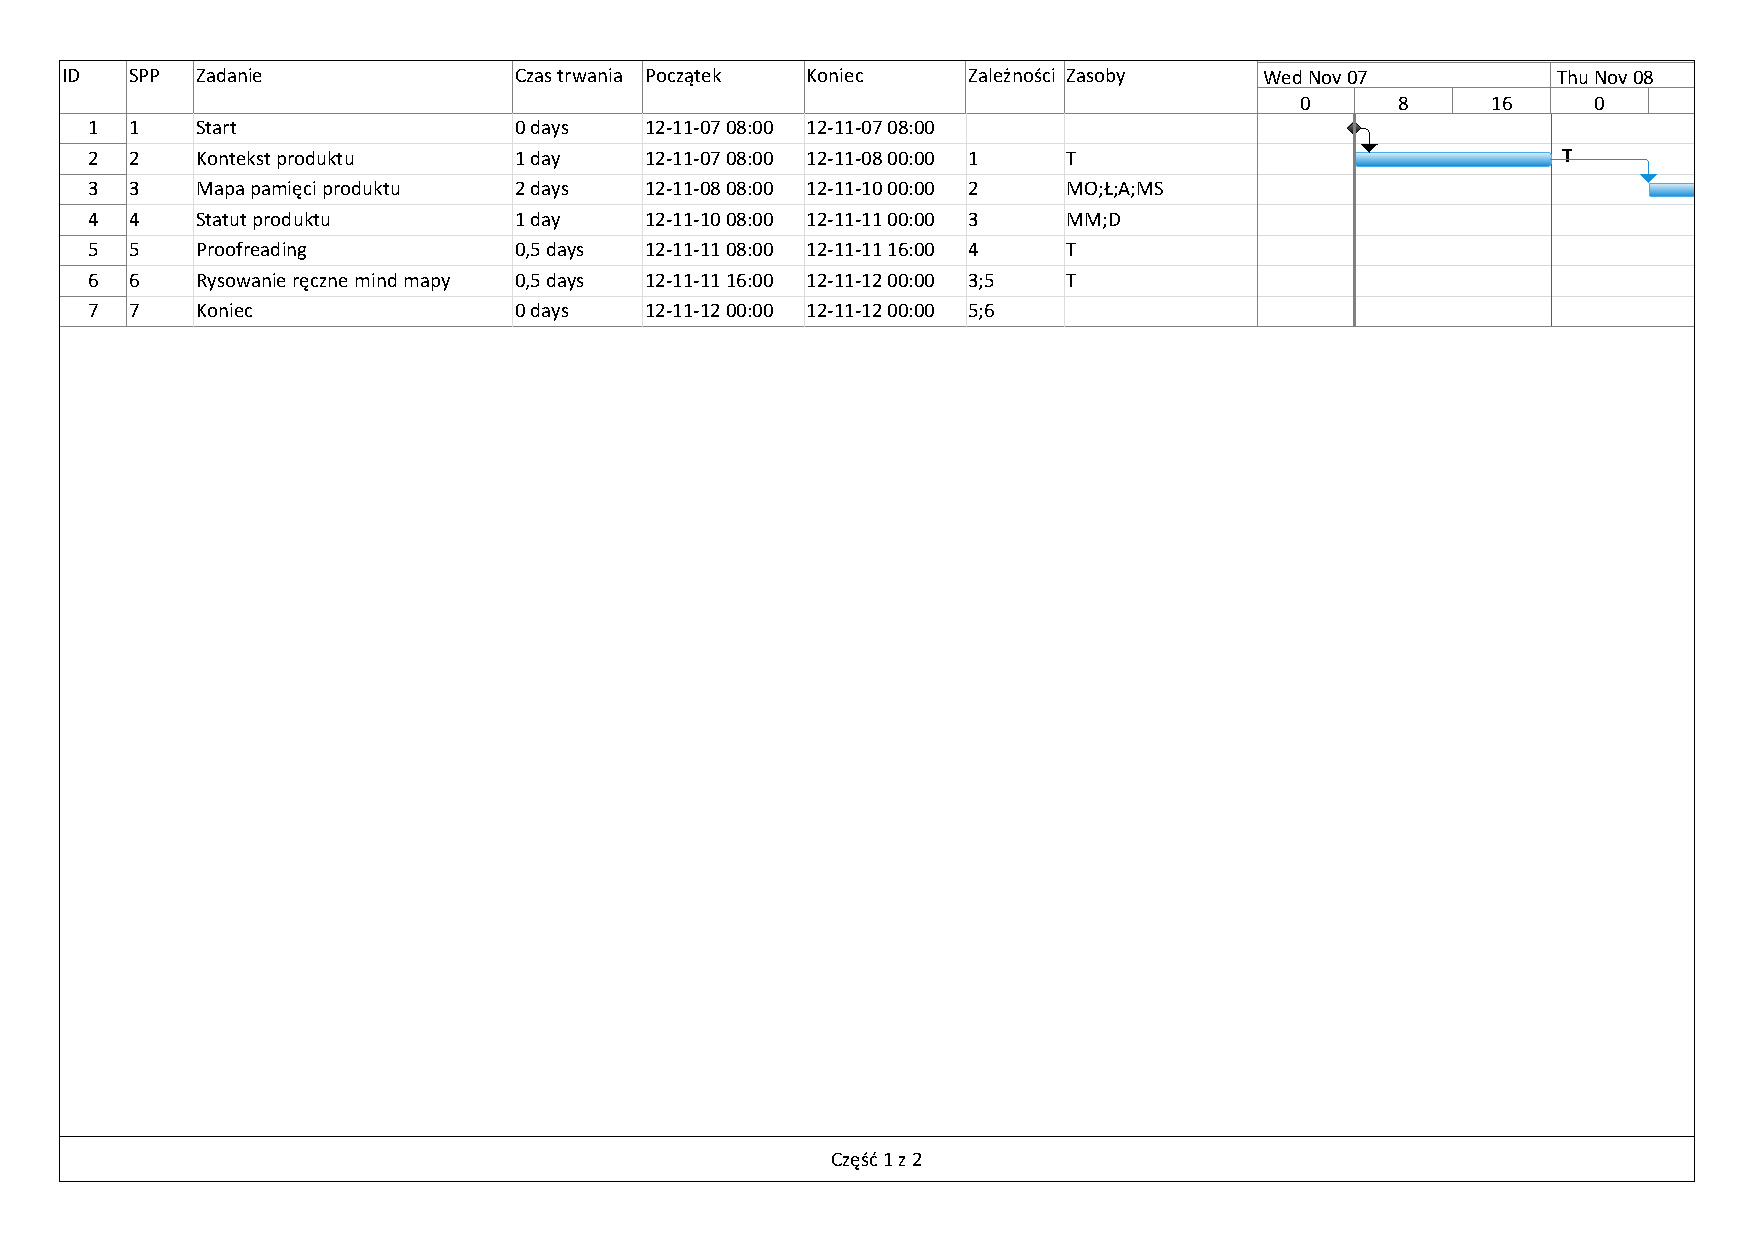
\includegraphics[page=1, trim=1cm 1cm 1cm 1cm, angle=270, width=\textwidth, clip=true]{./figury/harmonogram}
    \caption{Harmonogram pracy w ramach ćwiczenia 2.}
    \label{fig:harmonogram}
\end{figure}

\begin{figure}[p]
    \ContinuedFloat
    \includegraphics[page=2, trim=1cm 1cm 1cm 1cm, angle=270, width=\textwidth, clip=true]{./figury/harmonogram}
    \caption{Harmonogram pracy w ramach ćwiczenia 2. (kontynuacja)}
\end{figure}


\section{Historia dokumentu}
\begin{versions}
    \version*{1.0}{2012-11-07}{TC}%
        Dodano pełen harmonogram pracy.
    \version{1.1}{2012-11-07}{TC}%
        Poprawiono formatowanie.
    \version{1.2}{2012-11-07}{TC}%
        Usunięto zbędne elementy wygenerowane przez Microsoft Project.
\end{versions}


\end{document}
